%		 ** RISULTATI **

Le figure~\ref{fig:room} e~\ref{fig:console} mostrano un caso potenzialmente problematico di situazione ciclica. In tale situazione, tutti e quattro gli agenti della stanza sono occupati a tracciare un target diverso e l'inizio di un'asta potrebbe scatenare una reazione a catena senza fine. Utilizzando il protocollo d'asta implementato, la situazione si risolve con uno scambio di target.

% Figura della mappa
\begin{figure}[htp]
	\centering
	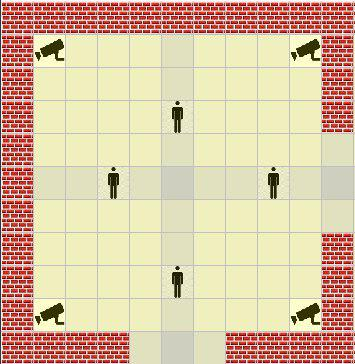
\includegraphics[width=0.3\linewidth]{room}
	\caption{Configurazione dei target ciclica.}
	\label{fig:room}
\end{figure}

% Figura della mappa
\begin{figure}[htp]
	\centering
	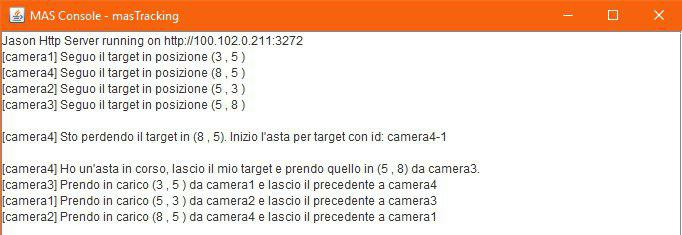
\includegraphics[width=0.7\linewidth]{console}
	\caption{Output ricevuto con la configurazione mostrata in Figura 3.}
	\label{fig:console}
\end{figure}

Le figure~\ref{fig:room2} e~\ref{fig:console2} mostrano un altro caso particolare. Nello scenario mostrato l'agente 2 vince l'asta per il target che l'agente 1 sta perdendo. Tuttavia, egli non riesce a cedere il suo attuale target e, di conseguenza, rifiuta la vincita. L'agente 1 allora ricalcola come vincitore l'agente 4, il quale riesce a cedere il suo attuale target ad un agente della stanza a fianco.

% Figura della mappa
\begin{figure}[htp]
	\centering
	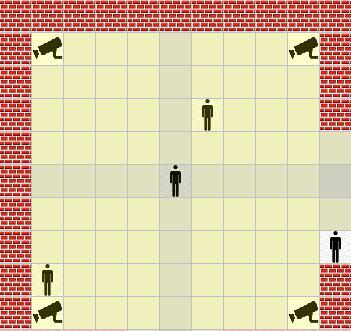
\includegraphics[width=0.3\linewidth]{room2}
	\caption{Configurazione dei target particolare.}
	\label{fig:room2}
\end{figure}

% Figura della mappa
\begin{figure}[htp]
	\centering
	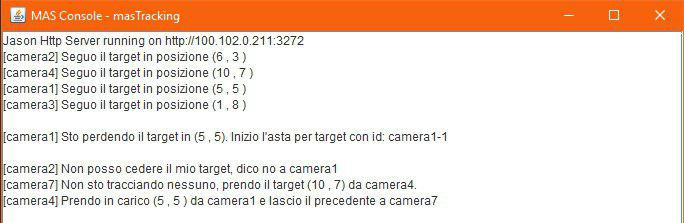
\includegraphics[width=0.7\linewidth]{console2}
	\caption{Output ricevuto con la configurazione mostrata in Figura 3.}
	\label{fig:console2}
\end{figure}

Le figure~\ref{fig:room3} e~\ref{fig:console3} mostrano il fallimento di un'asta. Infatti, tutti e tre i partecipanti candidati non possono cedere il proprio target. Il banditore mantiene quindi il proprio target nella speranza che rimanga ancora nel suo campo visivo.

% Figura della mappa
\begin{figure}[htp]
	\centering
	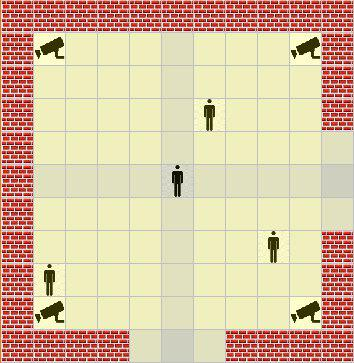
\includegraphics[width=0.3\linewidth]{room3}
	\caption{Configurazione dei target particolare.}
	\label{fig:room3}
\end{figure}

% Figura della mappa
\begin{figure}[htp]
	\centering
	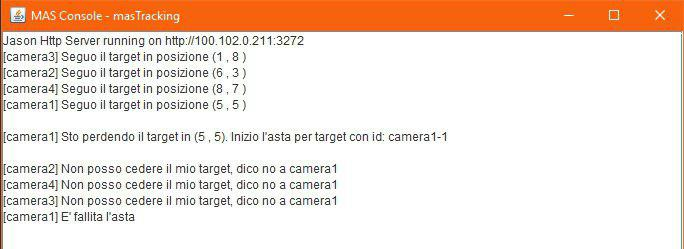
\includegraphics[width=0.7\linewidth]{console3}
	\caption{Output ricevuto con la configurazione mostrata in Figura 3.}
	\label{fig:console3}
\end{figure}

\newpage

La tabella seguente riassume, al variare del numero di target, le seguenti statistiche:
\begin{itemize}
	\item numero medio di aste effettuate,
	\item numero medio di aste non andate a buon fine,
	\item numero medio di step in cui un target non � tracciato.
\end{itemize}
\begin{center}
\begin{tabular}{| c | c | c | c |}
	\hline
	\textbf{No Target}	&	\textbf{No Aste}	&	\textbf{No Aste Fallite}	&	\textbf{No Target Persi} \\ \hline
	1	&	20	&	0	&	3	\\ \hline
	2	&	85	&	7	&	19	\\ \hline
	3	&	152	&	17	&	54	\\ \hline
	4	&	190	&	18	&	120	\\ \hline
	5	&	366	&	45	&	145	\\ \hline
\end{tabular}
\end{center}

I dati raccolti evidenziano come simulare con spazi stretti e aree di visione in comune piccole, porta gli agenti a perdere abbastanza spesso i loro target; soprattutto perch� questi hanno sviluppato una particolare abilit� a camminare sui bordi delle aree di visione.

In generale, per poter ottenere una stima migliore della bont� del sistema, bisognerebbe utilizzare un ambiente di simulazione con una risoluzione dello spazio maggiore. Inoltre, da un'analisi real time del comportamento del sistema stesso, � emersa la necessit� di una logica decisionale pi� intelligente per il riconoscimento dell'allontanamento dei target e della sua possibile perdita.